
\documentclass[11pt]{article}
\usepackage[utf8]{inputenc}
\usepackage{amsmath}
\usepackage{bm}
\usepackage{parskip}
\usepackage{listings}
\usepackage[margin=.8in]{geometry}
\setlength{\parindent}{0in}
\usepackage{indentfirst}
\usepackage{graphicx}
\usepackage{hyperref}
\usepackage{tikz}
\usetikzlibrary{arrows,shapes.arrows,positioning,shapes}
\usepackage{enumitem}
\usepackage{array}
\usepackage{arydshln}
\usepackage{booktabs}
\newcolumntype{M}[1]{>{\centering\arraybackslash}m{#1}}
\usepackage[english, cleanlook]{isodate}
\usepackage{setspace}
\setstretch{1.1}
\usepackage[round]{natbib}
\bibliographystyle{humannat-mod}
\usepackage{amsfonts}
\newcommand{\E}{{\rm I\kern-.3em E}}
\newcommand{\Var}{\text{Var}}
\newcommand{\V}{\text{V}}
\newcommand{\N}{\mathcal{N}}
\newcommand{\I}{\text{I}}
\newcommand{\Cov}{\text{Cov}}
\renewcommand{\P}{\text{P}}
\newcommand{\Cor}{\text{Cor}}
\newcommand{\logit}{\text{logit}}
\newcommand{\iid}{\stackrel{\text{iid}}{\sim}}
\newcommand{\bblue}[1]{\textbf{\textcolor{blue}{#1}}}
\newcommand{\bgreen}[1]{\textbf{\color{olive}{#1}}}
\usepackage{lscape}
\usepackage{soul,color}
\usepackage{rotating}
\usepackage[compact]{titlesec}
\usepackage[labelfont=bf]{caption}
\usepackage[hang]{footmisc}
\setlength\footnotemargin{0em}
\newcolumntype{R}[1]{>{\raggedleft\let\newline\\\arraybackslash\hspace{0pt}}m{#1}}
\def\arraystretch{1.3}
\usepackage{caption}
\captionsetup{labelfont={color=blue,bf}}

\title{\vspace{-1.5cm}Key topics in Soc 401/504: Advanced Social Statistics\\GLMs, maximum likelihood, and quantities of interest\vspace{-.9cm}}
\date{\vspace{-1.2cm}\small \begin{tabular}{p{.6\textwidth}p{.4\textwidth}}Last updated: \today & Ian Lundberg (ilundberg at princeton dot edu) \end{tabular}\vspace{-.3cm}}

\begin{document}

\maketitle

\section*{\textcolor{blue}{Defining GLMs}\footnote{For alternative presentations of GLMs, we recommend \citet{agresti2015} and \citet{powers2008}. A classic reference is \citet{mccullagh1989}. Handout color scheme inspired by \citet{efron2016}.}}

A \bgreen{generalized linear model} (GLM) extends the linear model to various response types: binary, count, ordinal, duration, etc. The \bgreen{data generating process} in a GLM involves three elements:

$$
\overbrace{\vec{X_i}\vec\beta = \eta_i}^\text{\bgreen{Linear predictor}} \qquad 
\overbrace{\eta_i = g(\mu_i)}^\text{\bgreen{Link function $g$}} \qquad 
\overbrace{Y_i \sim f_Y(\mu_i,\gamma)}^\text{\bgreen{Stochastic component}}
$$

GLMs are defined for data generated from distributions $f_Y$ in the \bgreen{exponential family} (see Supplement A). We use $\vec\theta$ to denote the full set of parameters to be estimated, which include coefficients $\vec\beta$ and, if relevant, a parameter $\gamma$ related to the variance. Table \ref{tbl:GLMs} provides examples of GLMs.

\section*{\bblue{Maximum likelihood}}

Unlike OLS, there is no general analytic formula for the optimal parameter estimates $\hat\beta$. Instead, we choose the parameters under which the data we observe would be most likely: we search for the parameters that maximize the \bgreen{likelihood}:\footnote{Maximum likelihood estimation has a close connection to Bayesian inference. See Supplement B.}
$$\overbrace{L\left(\vec\theta\mid \mathbf{X},\vec{y}\right)}^\text{Likelihood} = \overbrace{f_Y\left(\vec{y}\mid \mathbf{X}, \vec\theta\right)}^{\substack{\text{Probability density of}\\\text{data given parameters}}}$$
We often assume \bgreen{conditional independence}, thereby allowing us to factor the likelihood.
$$\begin{aligned}
L\left(\vec\theta\mid \mathbf{X},\vec{y}\right) &= f_Y\left(\vec{y}\mid \mathbf{X}, \vec\theta\right)
= f_Y\left(y_1\mid \vec{x}_1, \vec\theta\right)\times \dots\times f_Y\left(y_n\mid \vec{x}_n, \vec\theta\right)
= \prod_{i=1}^n f_Y\left(y_i\mid \vec{x}_i, \vec\theta\right)
\end{aligned}$$
Often, the likelihood factors. We can \bgreen{drop terms} that do not involve the parameters $\vec\theta$ to produce a function proportional to the likelihood; the value of $\vec\theta$ that maximizes the likelihood remains unchanged.
$$\begin{aligned}
L\left(\vec\theta\mid \mathbf{X},\vec{y}\right) &= \prod_{i=1}^n f_Y\left(y_i\mid \vec{x}_i, \vec\theta\right) 
= \prod_{i=1}^n h_1\left(y_i,\vec{x}_i\right)h_2\left(y_i, \vec{x}_i,\vec\theta\right) 
\propto \prod_{i=1}^n h_2\left(y_i, \vec{x}_i,\vec\theta\right)
\end{aligned}$$
The log is a monotone function, so the argument $\vec\theta$ that maximizes $L$ also maximizes the \bgreen{log likelihood}.
$$\begin{aligned}
\ell\left(\vec\theta\mid \mathbf{X},\vec{y}\right) &= \log L\left(\vec\theta\mid \mathbf{X},\vec{y}\right) 
= \log \left(\prod_{i=1}^n f_Y\left(y_i\mid \vec{x}_i, \vec\theta\right)\right) 
= \sum_{i=1}^n \log f_Y\left(y_i\mid \vec{x}_i, \vec\theta\right)
= \sum_{i=1}^n\log h_2\left(y_i, \vec{x}_i, \vec\theta\right) + c
\end{aligned}$$
where the constant $c = \sum_{i=1}^n h_1\left(y_i,\vec{x}_i\right)$ can be ignored.

\section*{\bblue{Climbing the mountain}}

The log likelihood is a mountain. Each point on the mountain is represented by coordinates that correspond to the parameter vector $\vec\theta$. We want to find the maximum likelihood estimate: the peak.

We will assume temporarily that the mountain has only one dimension: $\vec\theta=\theta$ has just one element.

The \bgreen{first derivative} $\frac{\partial}{\partial \theta}\ell\left(\theta\mid \mathbf{X},\vec{y}\right)$ captures the slope of the mountain. At the peak, the mountain is flat. We start by finding a candidate point $\theta^*$ at which the first derivative is 0.
$$\theta^* = \theta\text{ such that }\frac{\partial}{\partial \theta}\ell\left(\theta\mid \mathbf{X},\vec{y}\right) = 0$$

\begin{center}
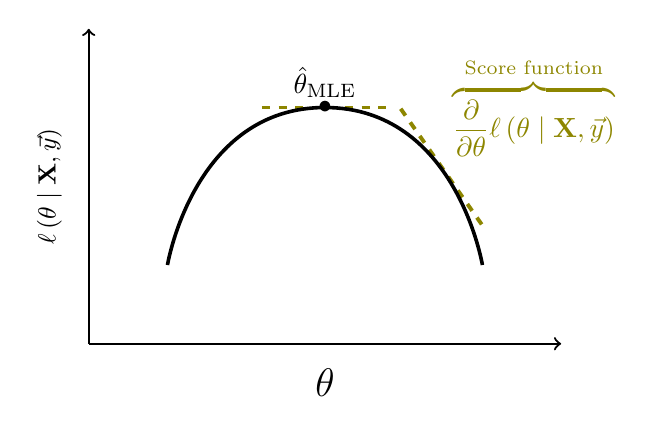
\begin{tikzpicture}
% Score function
\draw[olive, line width = 1.4pt, dashed, rotate = 35] (2.5,.1) -- (2.5,1.9); %(2,1.3) -- (0.5, 3);
\draw[olive, line width = 1.4pt, dashed] (-.8,3) -- (.8,3); %(2,1.3) -- (0.5, 3);
%\node[rotate = 305] at (2, 2.5) {$\frac{\partial}{\partial \theta}\ell(\theta\mid X,y)$};
\node[olive, anchor = west] at (1.5, 3) {$\overbrace{\frac{\partial}{\partial \theta}\ell\left(\theta\mid \mathbf{X},\vec{y}\right)}^\text{Score function}$};
% MLE
\node[anchor = south] (mleLabel) at (0,3) {$\hat\theta_\text{MLE}$};
\node[fill=none] (mle) at (0,3) {$\bullet$};
% Curve
\draw[line width = 1.3] plot [smooth,tension=1.5] coordinates {(-2,1) (mle.center) (2,1)};
% Axes
\draw[->, thick] (-3, 0) -- (-3, 4);
\draw[->, thick] (-3, 0) -- (3, 0);
\node at (0,-.5) {\Large $\theta$};
\node[rotate=90] at (-3.5,2) {\small $\ell\left(\theta\mid \mathbf{X},\vec{y}\right)$};
\end{tikzpicture}
\end{center}

If $\vec\theta$ has many elements, the first derivative is called the \bgreen{gradient} (denoted $\nabla$) and captures the slope along each coordinate. The gradient is also called the \bgreen{score function}.

$$\nabla \ell\left(\vec\theta\mid \mathbf{X},\vec{y}\right) = \begin{bmatrix}
\frac{\partial}{\partial \theta_1}\ell\left(\vec\theta\mid \mathbf{X},\vec{y}\right) \\ 
\vdots \\ 
\frac{\partial}{\partial \theta_p}\ell\left(\vec\theta\mid \mathbf{X},\vec{y}\right) 
\end{bmatrix}$$

In the multivariate case, a place where every element of the score vector is 0 is a candidate peak.

A flat place could be a peak or a valley. To see whether we have found a maximum, we take the \bgreen{second derivative} and evaluate it at our candidate $\theta^*$. It tells us the direction of the curvature.

\begin{center}
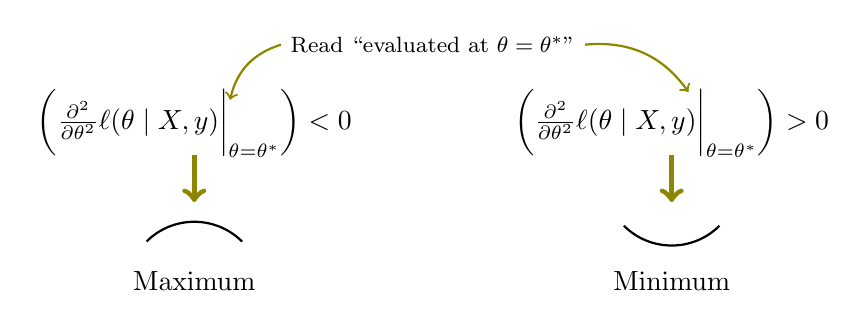
\begin{tikzpicture}[x = .25\textwidth, y = 1cm]
\node (explanation) at (0,3) {\footnotesize Read ``evaluated at $\theta = \theta^*$''};
\draw[->, thick, olive] (explanation.west) to[bend right] (-.85,2.3);
\draw[->, thick, olive] (explanation.east) to[bend left] (1.07,2.4);
\node (negative) at (-1,2) {$\bigg(\frac{\partial^2}{\partial \theta^2}\ell(\theta\mid X,y)\bigg\rvert_{\theta = \theta^*}\bigg) < 0$};
\node (positive) at (1,2) {$\bigg(\frac{\partial^2}{\partial \theta^2}\ell(\theta\mid X,y)\bigg\rvert_{\theta = \theta^*}\bigg) > 0$};
\draw[->, olive, line width = 2pt] (-1,1.6) -- (-1, 1);
\draw[->, olive, line width = 2pt] (1,1.6) -- (1, 1);
\draw[thick] (-1.2,.5) to[bend left = 45] (-.8, .5);
\draw[thick] (1.2,.7) to[bend left = 45] (.8, .7);
\node at (-1,0) {Maximum};
\node at (1,0) {Minimum};
\end{tikzpicture}
\end{center}

If the first derivative is 0 and the second derivative is negative, then $\theta^*$ is our \bgreen{maximum likelihood estimate} $\hat\theta_\text{MLE}$.\footnote{Technical note: In GLMs, the objective function is convex so there is no risk of a local maximum; there is only one maximum. In more complex models you may worry whether your maximum is a global maximum.}

When $\vec\theta$ has many dimensions, we get a matrix of second derivatives called the \bgreen{Hessian}.

$$H = \nabla \nabla^T \ell\left(\vec{\theta}\mid \mathbf{X},\vec{y}\right) = \begin{small}\begin{bmatrix}
\frac{\partial^2}{\partial \theta_1^2}\ell\left(\vec{\theta}\mid \mathbf{X},\vec{y}\right) & 
	\frac{\partial}{\partial \theta_1}\frac{\partial}{\partial \theta_2}\ell\left(\vec{\theta}\mid \mathbf{X},\vec{y}\right) & 
	\cdots & 
	\frac{\partial}{\partial \theta_1}\frac{\partial}{\partial \theta_p}\ell\left(\vec{\theta}\mid \mathbf{X},\vec{y}\right) \\ 
\frac{\partial}{\partial \theta_1}\frac{\partial}{\partial \theta_2}\ell\left(\vec{\theta}\mid \mathbf{X},\vec{y}\right) &
	\frac{\partial^2}{\partial \theta_2^2}\ell\left(\vec{\theta}\mid \mathbf{X},\vec{y}\right) &
	\cdots &
	\frac{\partial}{\partial \theta_2}\frac{\partial}{\partial \theta_p}\ell\left(\vec{\theta}\mid \mathbf{X},\vec{y}\right) \\
\vdots & \vdots & \ddots & \vdots \\
\frac{\partial}{\partial \theta_1}\frac{\partial}{\partial \theta_p}\ell\left(\vec{\theta}\mid \mathbf{X},\vec{y}\right) &
	\frac{\partial}{\partial \theta_2}\frac{\partial}{\partial \theta_p}\ell\left(\vec{\theta}\mid \mathbf{X},\vec{y}\right) &
	\cdots &
	 \frac{\partial^2}{\partial \theta_p^2}\ell\left(\vec{\theta}\mid \mathbf{X},\vec{y}\right) \\ 
\end{bmatrix}\end{small}$$

\section*{\bblue{Variance of $\hat\theta_\text{MLE}$}}

The variance of the MLE estimator relates to the amount of curvature at the peak: the Hessian.

Heuristically, a very negative Hessian at the MLE (the peak) suggests that the score changes quickly from positive to negative near the MLE; we have a lot of information about the MLE. For this reason, the negative Hessian is called the \bgreen{Fisher information}.

The \bgreen{variance of the MLE estimate} is the inverse of the Fisher information:
$$\V\left(\hat\theta_{\text{MLE}}\right) = \bigg(\mathcal{I}_n(\theta)\bigg)^{-1}\bigg\rvert_{\theta = \theta_\text{MLE}}$$
In practice, we don't know the true $\theta$, so we estimate the variance by evaluating the inverse Fisher information at our MLE estimate. This is sometimes called the observed Fisher information.
$$\hat\V\left(\hat\theta_{\text{MLE}}\right) = \bigg(\mathcal{I}_n(\theta)\bigg)^{-1}\bigg\rvert_{\theta = \hat\theta_\text{MLE}}$$

\bgreen{Remember:} Sharper peak $\rightarrow$ more negative Hessian $\rightarrow$ more positive Fisher information $\rightarrow$ lower variance estimate

\section*{\bblue{Properties of the MLE\footnote{For more details on inference on MLE theory, we recommend \citet{casella2002}. Invariance is Thm. 7.2.10, consistency is Thm. 10.1.6, normality is Thm. 10.1.12, the CRLB is Thm. 7.3.9, and asymptotic efficiency is defined in Def. 10.1.11 and related to MLE in Thm. 10.1.12.}}}
\begin{enumerate}
\item \bgreen{Invariance}: If $\hat{\vec\theta}_\text{MLE}$ is the MLE for $\vec\theta$, then for any function $g(\vec\theta)$ the MLE of $g(\vec\theta)$ is $g(\hat{\vec\theta}_\text{MLE})$.
\item \bgreen{Consistency:} The MLE is sometimes biased $\left(\E\left[\hat{\vec\theta}_\text{MLE}\right]\neq \vec\theta\right)$ but is always consistent: $\hat{\vec\theta}_\text{MLE}\stackrel{P}{\rightarrow}\vec\theta$.
\item \bgreen{Asymptotic normality}: As $n\rightarrow\infty$, the sampling distribution of $\hat\theta_\text{MLE}$ converges to Normal.
\vspace{-2ex}$$\sqrt{n}\left(\hat{\vec\theta} - \vec{\theta}\right) \stackrel{D}{\rightarrow} \text{Normal}\left(0,\left[\mathcal{I}_1(\theta)\right]^{-1}\right)$$ \vspace{-6ex}
% Commenting this alternative version out because really \hat{\vec\theta} converges in probability to \theta,
% so it's clearer to multiply by \sqrt{n} on the left and use the Fisher information from a single observation on the right.
%$$\hat{\vec\theta} \stackrel{D}{\rightarrow} \text{Normal}\left(\theta,\V\left[\hat{\vec\theta}_\text{MLE}\right]\right)$$
\item \bgreen{Efficiency:} The Cram\'{e}r-Rao lower bound states that any unbiased estimator for $\vec{\theta}$ has variance at least as great as $\left(\mathcal{I}_n(\theta)\right)^{-1}$, which is $\V\left(\hat{\vec\theta}_\text{MLE}\right)$. This means:
\begin{itemize}
\item If the MLE is unbiased, it is the most efficient (lowest variance) among unbiased estimators. However, the MLE is often biased.
\item The MLE is asymptotically efficient: even biased MLEs asymptotically achieve the CRLB.
\end{itemize}
\end{enumerate}

\newpage
\section*{\bblue{Hypothesis testing\footnote{These tests can be generalized to the null hypothesis $H_0: h(\vec\theta\,) = \vec{c}$, where $h$ is a function that maps the vector $\vec\theta\in\mathbb{R}^p$ to a vector of constraints $c\in \mathbb{R}^k$. For an overview in this more general framework, see \citet{rao2005}. For a textbook treatment including a discussion of inverting the tests to produce confidence intervals, see \citet{agresti2015} Section 4.3.}}}
Suppose we want to test the null hypothesis that a subset of the coefficients are zero.
$$\vec\beta = \begin{bmatrix} \vec\beta_A \\ \vec\beta_B \end{bmatrix},\qquad H_0: \vec\beta = \vec\beta_0 \equiv \begin{bmatrix} \vec{0} \\ \vec\beta_B \end{bmatrix}$$
There are three main methods for conducting this test. We will denote the number of elements in $\vec\theta_A$ by $k$, often using the $k=1$ case to build intuition. %Figure \ref{fig:tests} also builds intuition in the case of $k = 1$.

%\begin{figure}[!ht]
\begin{center}
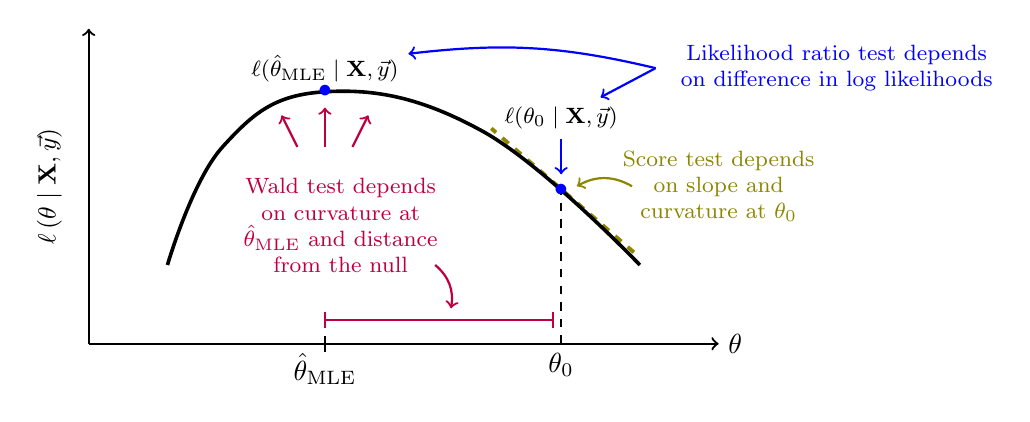
\begin{tikzpicture}
% Score test
\node[olive, font = \footnotesize,align = center] at (5, 2) {Score test depends\\on slope and\\curvature at $\theta_0$};
\draw[olive, line width = 1.4pt, dashed, rotate = 49] (3.45,-2.2) -- (3.45,.2);
\draw[->, thick, olive] (3.9,2) to[bend right] (3.2,2);
% Wald test
\node[purple, font = \footnotesize,align = center] at (0.2,1.5) {Wald test depends\\on curvature at\\$\hat\theta_\text{MLE}$ and distance\\from the null};
\draw[->, thick, purple] (0,2.5) -- (0,3);
\draw[->, thick, purple] (-.35,2.5) -- (-.55,2.9);
\draw[->, thick, purple] (.35,2.5) -- (.55,2.9);
\draw[-, thick, purple] (0,.3) -- (2.9,.3);
\draw[-, thick, purple] (0,.2) -- (0,.4);
\draw[-, thick, purple] (2.9,.2) -- (2.9,.4);
\draw[->, thick, purple] (1.4,1) to[bend left] (1.6,.45);
% Curve
\draw[line width = 1.3] plot [smooth,tension=.7] coordinates {(-2,1) (-1.3,2.5) (0,3.2) (2,2.7) (4,1)};
% MLE
\node[anchor = south,font = \footnotesize] (mleLabel) at (0,3.2) {$\ell(\hat\theta_\text{MLE}\mid \mathbf{X},\vec{y})$};
\node[fill=none,blue] (mle) at (0,3.2) {$\bullet$};
% Null hypothesis
\node[anchor = south,font = \footnotesize] (nullLabel) at (3,2.6) {$\ell(\theta_0\mid \mathbf{X},\vec{y})$};
\node[fill=none,blue] (null) at (3,1.95) {$\bullet$};
\draw[->, thick, blue] (nullLabel) -- (null);
% Likelihood ratio test
\node[blue, font = \footnotesize,align = center] at (6.5,3.5) {Likelihood ratio test depends\\on difference in log likelihoods};
\draw[->, thick, blue] (4.2,3.5) to[bend right = 10] (mleLabel);
\draw[->, thick, blue] (4.2,3.5) -- (nullLabel);
% Axes
\draw[->, thick] (-3, 0) -- (-3, 4);
\draw[->, thick] (-3, 0) -- (5, 0);
\node[anchor=north] at (0,0) {$\hat\theta_\text{MLE}$};
\draw[-, thick] (0, -.1) -- (0, .1);
\node[anchor=west] at (5,0) {$\theta$};
\node[rotate=90] at (-3.5,2) {\small $\ell\left(\theta\mid \mathbf{X},\vec{y}\right)$};
\node[anchor=north] at (3,0) {$\theta_0$};
\draw[thick, dashed] (3,0) -- (3,1.9);
\end{tikzpicture}
\end{center}
%\caption{Intuition for Wald, score, and likelihood ratio tests with one parameter}
%\label{fig:tests}
%\end{figure}

The \bgreen{Wald test} \citep{wald1943} relies on the asymptotic normality of $\hat\beta_\text{MLE}$:

\begin{center}
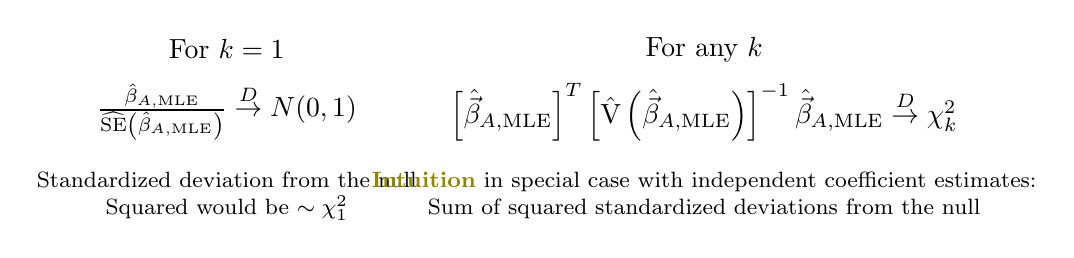
\begin{tikzpicture}[x = .25\textwidth, y = .8cm]
\node at (-1,1) {For $k=1$};
\node at (1,1) {For any $k$};
\node at (-1,0) {$\frac{\hat\beta_{A,\text{MLE}}}{\widehat{\text{SE}}\left(\hat\beta_{A,\text{MLE}}\right)} \stackrel{D}{\rightarrow} N(0,1)$};
\node at (1,0) {$\left[\hat{\vec\beta}_{A,\text{MLE}}\right]^T
	\left[\hat\V\left(\hat{\vec{\beta}}_{A,\text{MLE}}\right)\right]^{-1}
	\hat{\vec\beta}_{A,\text{MLE}}
	\stackrel{D}{\rightarrow} \chi^2_k$};
\node[align=center,anchor=north,font=\footnotesize] at (-1,-.8) {Standardized deviation from the null\\Squared would be $\sim \chi^2_1$};
\node[align=center,anchor=north,font=\footnotesize] at (1,-.8) {\bgreen{Intuition} in special case with independent coefficient estimates:\\Sum of squared standardized deviations from the null};
\end{tikzpicture}
\end{center}

The \bgreen{likelihood ratio test} \citep{neyman1933,wilks1938} compares nested models: a restricted model estimating $\vec\beta_B$ and assuming $\vec\beta_A=0$ with likelihood $L^*_R$, and an unrestricted model with likelihood $L^*$.%\footnote{See \citet{casella2002} Thm. 10.3.1.}

\begin{center}
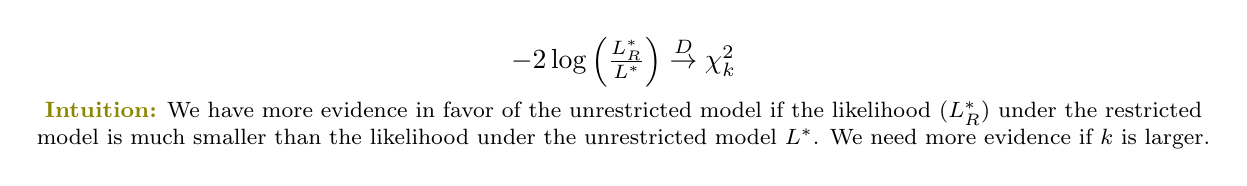
\begin{tikzpicture}[x = .25\textwidth, y = .8cm]
\node at (0,0) {$-2\log\left(\frac{L^*_R}{L^*}\right) \stackrel{D}{\rightarrow} \chi^2_k$};
\node[align=center,font=\footnotesize] at (0,-1) {
	\bgreen{Intuition:} We have more evidence in favor of the unrestricted model if the likelihood ($L^*_R$) under the restricted\\
	 model is much smaller than the likelihood under the unrestricted model $L^*$. We need more evidence if $k$ is larger.
};
\end{tikzpicture}
\end{center}

The \bgreen{score test} \citep{rao1948} is based on the score function and the Fisher information evaluated at $\vec\beta_0$.

\begin{center}
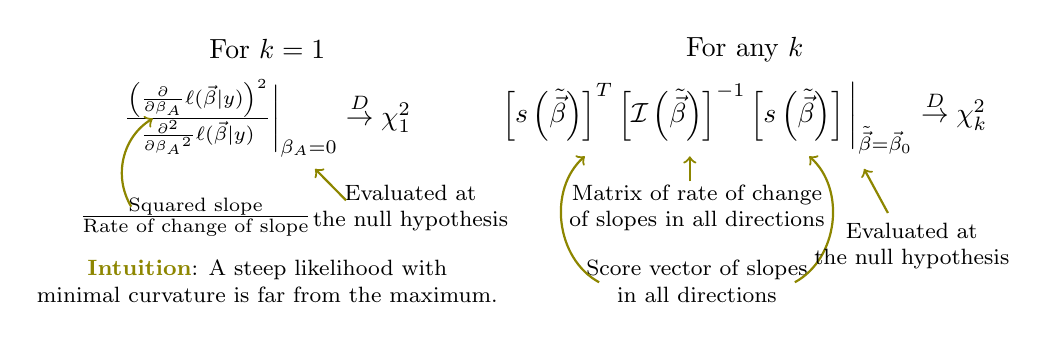
\begin{tikzpicture}[x = .25\textwidth, y = .8cm]
\node at (-1,1.1) {For $k=1$};
\node at (1,1.1) {For any $k$};
\node at (-1,0) {$\frac{\left(\frac{\partial}{\partial \beta_A}\ell(\vec\beta\mid y)\right) ^ 2}
	{\frac{\partial^2}{\partial {\beta_A}^2}\ell(\vec\beta\mid y)}
	\bigg\rvert_{\beta_A = 0}
	\stackrel{D}{\rightarrow} \chi^2_1$};
\node at (1,0) {$\left[s\left(\tilde{\vec\beta}\right)\right]^T
	\left[\mathcal{I}\left(\tilde{\vec\beta}\right)\right]^{-1}
	\left[s\left(\tilde{\vec\beta}\right)\right]\bigg\rvert_{\tilde{\vec\beta} = \vec\beta_0}
	\stackrel{D}{\rightarrow} \chi^2_k$};
\node[align=center,anchor=north] at (-1.3,-1.1) {$\frac{\text{Squared slope}}{\text{Rate of change of slope}}$};
\draw[->, thick, olive] (-1.57,-1.4) to[bend left = 45] (-1.48,0);
\node[align=center,anchor=north,font=\footnotesize] at (-.4,-.9) {Evaluated at\\the null hypothesis};
\draw[->, thick, olive] (-.67,-1.3) -- (-.8,-.8);
\node[align=center,anchor=north,font=\footnotesize] at (-1,-2.1) {\bgreen{Intuition}: A steep likelihood with\\minimal curvature is far from the maximum.};
\node[align=center,anchor=north,font=\footnotesize] at (.8,-.9) {Matrix of rate of change\\of slopes in all directions};
\node[align=center,anchor=north,font=\footnotesize] at (.8,-2.1) {Score vector of slopes\\in all directions};
\draw[->, thick, olive] (.39,-2.6) to[bend left = 55] (.33,-.6);
\draw[->, thick, olive] (1.21,-2.6) to[bend right = 55] (1.27,-.6);
\draw[->, thick, olive] (0.77,-1) -- (0.77,-.6);
\node[align=center,anchor=north,font=\footnotesize] at (1.7,-1.5) {Evaluated at\\the null hypothesis};
\draw[->, thick, olive] (1.6,-1.5) -- (1.5,-.8);
\end{tikzpicture}
\end{center}

\section*{\bblue{Reporting results}}

The parameters $\vec\theta$ are rarely of interest; regression coefficients are always difficult to interpret. Instead, you should always report \bgreen{quantities of interest} that clearly summarize your finding.\footnote{This strategy was originally advocated by \citet{king2000}. Some functions to fit common GLMs are available in the \texttt{Zelig} package in \texttt{R} \citep{imai2008,choirat2017}.} These might include predicted probabilities, first differences, the average treatment effect, etc.

The entire process can be summarized in a few simple steps:
\begin{enumerate}
\item \bgreen{Fit a model}. Assume a model, write the log likelihood, and estimate $\hat\theta_\text{MLE}$ and the Hessian.
\item \bgreen{Simulate estimation uncertainty}. We are uncertain about the true MLE $\vec\theta$. We want to incorporate this uncertainty in our estimate. We approximate the sampling distribution of $\hat{\vec\theta}_\text{MLE}$ with thousands of draws from a multivariate normal distribution.\footnote{It is important that all parameters are simulated together $\left(\tilde{\vec\theta}\text{ includes both }\tilde{\vec\beta}\text{ and }\tilde\gamma\right)$.}\footnote{The log likelihood is asymptotically normal. The proof invokes the Central Limit Theorem and the fact that the log likelihood is a sum of independent quantities. Draws from the likelihood are the likelihoodist analog of draws from the posterior distribution in Bayesian inference. For more on the likelihood theory of inference, see \citet{king1998}.}
$$\tilde\theta \sim N\left(\hat{\vec\theta}_\text{MLE},\underbrace{\hat\V\left(\hat{\vec\theta}_\text{MLE}\right)}_\text{Variance-covariance matrix}\right)$$
\item \bgreen{Calculate the linear predictor} for each observation for each draw. Depending on your quantity of interest, you may want to change the $\vec{X}_i$ values of some observations so that the observations you compare are informative for your theory. $$\left\{\tilde\eta_i = \vec{X}_i\tilde{\vec\beta}\right\}_{i=1}^n$$
\item Transform by the \bgreen{inverse link function}. $\left\{\tilde\mu_i = g^{-1}\left(\tilde\eta_i\right)\right\}_{i=1}^n$
\begin{itemize}
\item The link function is $g(\mu_i) = \vec{X}_i\vec\beta$. The inverse link function does the reverse: $\mu_i = g^{-1}\left(\vec{X}_i{\vec\beta}\right)$.
\end{itemize}
\item \bgreen{Simulate fundamental uncertainty}. Even if we knew the true $\vec\theta$, a component would remain that is fundamentally stochastic. Draw from the distribution of $Y$ to simulate this.
$$\left\{\tilde{Y}_i \sim f_Y\left(\tilde\mu_i,\tilde\gamma\right)\right\}_{i=1}^n$$
\item \bgreen{Calculate your quantity of interest}. This is the thing you want to report to your readers.
$$\tilde\tau = \overbrace{h\left(\tilde{Y}_1,\dots,\tilde{Y}_n\right)}^{\substack{\text{Any quantity you}\\\text{want to report}}}$$
\item \bgreen{Repeat} steps 2-6 thousands of times.
\item \bgreen{Summarize} the resulting distribution of the $\tilde\tau$ samples in a clear, informative graph. 
\end{enumerate}

% \section*{\bblue{Comparing models}}

% Deviance. Cross-validation. 

\begin{sidewaystable}[!htbp]
\small
\centering
\begin{tabular}{lcccccc}
 & & Unknown & Linear \\
Model & Response type & parameters & predictor & = & Link function $g$ & Stochastic component \\
\hline

OLS & 
	Normal & 
	$\vec\theta=\left\{\vec\beta,\gamma\right\}$ & 
	$\vec{X}_i\vec\beta=\eta_i$ & 
	= &
	$g(\mu_i) = \mu_i$ & 
	$Y_i \sim \text{Normal}(\mu_i,\sigma^2 = \gamma)$ \\

Logit & 
	Binary & 
	$\vec\theta=\vec\beta$ & 
	$\vec{X}_i\vec\beta=\eta_i$ & 
	= &
	$g(\mu_i) = \logit(\mu_i) = \log\left(\frac{\mu_i}{1-\mu_i}\right)$ & 
	$f_Y(\mu_i) = \text{Bernoulli}(\pi_i = \mu_i)$ \\

Probit & 
	Binary & 
	$\vec\theta=\vec\beta$ & 
	$\vec{X}_i\vec\beta=\eta_i$ & 
	= &
	$g^*(\mu_i) = \text{probit}(\mu_i) = \Phi^{-1}(\mu_i)$ & 
	$Y_i \sim \text{Bernoulli}(\pi_i = \mu_i)$ \\
	
Complementary log-log & 
	Binary & 
	$\vec\theta=\vec\beta$ & 
	$\vec{X}_i\vec\beta=\eta_i$ & 
	= &
	$g^*(\mu_i) = \log(-\log(1-\mu_i)) $ & 
	$Y_i \sim \text{Bernoulli}(\pi_i = \mu_i)$ \\
	
Poisson & 
	Count & 
	$\vec\theta=\vec\beta$ & 
	$\vec{X}_i\vec\beta=\eta_i$ & 
	= &
	$g(\mu_i) = \log(\mu_i)$ & 
	$Y_i \sim \text{Poisson}(\lambda_i = \mu_i)$ \\

Neg. Binomial & 
	Count & $\vec\theta=\left\{\vec\beta,\gamma\right\}$ & 
	$\vec{X}_i\vec\beta=\eta_i$ & 
	= &
	$g^*(\mu_i) = \log(\mu_i)$ & 
	$Y_i \sim \text{NegBin}\left(\gamma, \pi_i = \frac{\mu_i}{\gamma + \mu_i}\right)$ \\

Exponential & 
	Duration & 
	$\vec\theta=\vec\beta$ & 
	$\vec{X}_i\vec\beta=\eta_i$ & 
	= &
	$g^*(\mu_i) = \log\left(\frac{1}{\mu_i}\right) = \log\left(\lambda_i\right)$ & 
	$Y_i \sim \text{Exponential}\left(\lambda_i = \frac{1}{\mu_i}\right)$ \\
	
	& & & & & $g(\mu_i) = \frac{1}{\mu_i} = \lambda_i$ \\

% Weibull and Gompertz could be added

Gamma & 
	Duration & 
	$\vec\theta=\left\{\vec\beta,\gamma\right\}$ & 
	$\vec{X}_i\vec\beta=\eta_i$ & 
	= &
	$g^*(\mu_i) = \log\left(\frac{1}{\mu_i}\right) = \log\left(\lambda_i\right)$ & 
	$Y_i \sim \text{Gamma}\left(\alpha = \gamma, \lambda_i = \frac{\gamma}{\mu_i}\right)$ \\
	
	& & & & & $g(\mu_i) = \frac{1}{\mu_i} = \lambda_i$ \\
	
Multinomial logit &
	Categorical & 
	$\bm{\theta}=\bm\beta=\left[\vec\beta_2 \cdots \vec\beta_k\right]$ &
	$\vec{X_i}\bm{\beta} = \vec\eta_i$ & 
	= &
	$g(\vec\mu_i) = \log\left(\frac{\vec{\mu}_i}{1 - \vec\mu_i^T\vec{1}}\right)$ &
	$Y_i \sim \text{Multinomial}\left(\vec\pi_i = \begin{bmatrix} 1 - \vec\mu_i^T \vec{1} \\ \vec\mu_i\end{bmatrix}\right)$ \\

%Multinomial probit could be added
	
%Ordered logit could be added
	
%Ordered probit could be added
	
\hline
\end{tabular}
\caption{Common generalized linear models (GLMs). List is not exhaustive. Alternative parameterizations and link functions exist; these were chosen to maximize consistency of notation within the table. Link functions denoted $g^*$ are not the canonical link for the given response type (see Supplement A). There are various reasons to choose a non-canonical link in some cases; one such reason is that the inverse of the canonical link $g^{-1}(\eta_i) = \mu_i$ does not always map all possible values of $\eta_i$ (the real line) into the support of $\mu_i$.}
\label{tbl:GLMs}
\end{sidewaystable}

\newpage
\appendix

\section*{\bblue{Supplement A. Exponential family}}
\label{exponentialFamily}
The distributions used in generalized linear models all come from the \bgreen{exponential family}. \\ The probability density function of each distribution can be written in the following form:
$$f(y\mid \vec\theta) = \overbrace{h(y)}^{\substack{\text{Normalizing}\\\text{constant}}} \exp\bigg(\overbrace{{\vec\theta}^T}^{\substack{\text{Natural}\\\text{parameter}}}\overbrace{\vec\phi(y)}^{\substack{\text{Sufficient}\\\text{statistics}}} - \overbrace{A\left(\vec\theta\right)}^{\substack{\text{Cumulant}\\\text{function}}}\bigg)$$
\bgreen{Ex.} For the Bernoulli,
$$\begin{aligned}
P(y\mid p) &= \pi^y(1-\pi)^{1-y} \\
&= \exp\bigg(\log\left(\pi^y(1-\pi)^{1-y}\right)\bigg) \\
&= \exp\bigg(y\log(\pi) + (1 - y)\log(1 - \pi)\bigg) \\
&= \exp\bigg(\underbrace{y}_{=\phi(y)}\underbrace{\log\left(\frac{\pi}{1-\pi}\right)}_{=\theta} + \underbrace{\log(1 - \pi)}_{=\log(1 - \logit^{-1}[\theta]) = -A(\theta)}\bigg)
\end{aligned}$$
The \bgreen{canonical link function} is the one that transforms the mean of the distribution to the natural parameter $\theta$. In this case, the canonical link function is $g(\pi) = \log\left(\frac{\pi}{1-\pi}\right) = \logit(\pi)$. This is why the logit is popular!

The exponential family is nice because:
\begin{enumerate}
\item Sufficient statistics $\vec\phi(y)$ are finite in dimension even in an infinite sample. To calculate the MLE, you only need the sufficient statistics and not actually all of the data. Information is compressed.
\item Conjugate priors exist for Bayesian inference.
\item The exponential family has maximum entropy (most diffuse) among distributions subject to some moment constraints.
\item The mean has a known formula: $\E(Y) = \nabla A(\theta)$. For the Bernoulli example, 
$$\begin{aligned}
\E(Y) &= \nabla A(\theta) \\
&= \frac{\partial}{\partial \theta} \bigg[-\log(1 - \logit^{-1}[\theta])\bigg] \\
&= \frac{\partial}{\partial \theta} \bigg[-\log\left(\frac{1}{1 + e^{\theta}}\right)\bigg] \\
&= -\bigg(\left(1 + e^{\theta}\right)\left(-e^\theta \left[1 + e^\theta\right]^{-2}\right)\bigg) \\
&= \left(\frac{e^\theta}{1 + e^\theta}\right) \\
&= \pi
\end{aligned}$$
\item The variance has a known formula: $\V(Y) = \nabla \nabla^T A(\theta)$. For the Bernoulli example,
$$\begin{aligned}
\V(Y) &= \nabla \nabla^T A(\theta) \\
&= \frac{\partial^2}{\partial^2 \theta} \bigg[-\log(1 - \logit^{-1}[\theta])\bigg] \\
&= \frac{\partial}{\partial \theta} \left(\frac{e^\theta}{1 + e^\theta}\right) \\
&= \frac{e^\theta}{\left(1 + e^\theta\right)^2} \\
&= \left(\frac{e^\theta}{1 + e^\theta}\right)\left(\frac{1}{1 + e^\theta}\right) \\
&= \pi(1 - \pi)
\end{aligned}$$
\end{enumerate}

For more complex distributions, having a known function for the mean and variance is nice! For more on the exponential family, we recommend \citet{murphy2012} Ch. 9. A Bayesian technique called \bgreen{variational inference} approximates distributions with the closest possible match among the exponential family (see \citealt{murphy2012} Ch. 21). There are also many fun connections between the distributions within the exponential family; for this we recommend \citet{blitzstein2014}.

\section*{\bblue{Supplement B. Connection to Bayesian inference}}
\label{bayes}
We will not cover Bayesian inference in this class. In this class, the unknown parameters ($\beta$) are treated as fixed constants. In Bayesian inference, the unknown parameters are treated as random variables.
$$P(\vec\theta\mid \vec{y}) = \frac{\overbrace{P(\vec{y}\mid \vec\theta)}^\text{Likelihood}\overbrace{P(\vec\theta)}^\text{Prior}}{\underbrace{P(\vec{y})}_\text{Normalizing constant}}$$
Because the normalizing constant does not involve the unknown parameters $\theta$, we can ignore it. The two key components in Bayesian inference are the \bgreen{prior distribution} on the unknown parameters and the \bgreen{likelihood}. What you learn about likelihood in this course will prepare you to jump into Bayesian inference in the future.

As an example of Bayesian inference, consider Bernoulli draws for which we assume a $\text{Beta}(\alpha,\beta)$ prior on the probability of success $\pi$. This corresponds to our beliefs about the distribution of $\pi$ before seeing the data.
$$\begin{aligned}
\pi &\sim \text{Beta}(\alpha,\beta) \\
Y_i &\stackrel{\text{iid}}{\sim} \text{Bernoulli}(\pi_i)
\end{aligned}$$
Bayesian inference produces a \bgreen{posterior distribution} that summarizes our updated beliefs given the data. In the Bernoulli case, the Beta distribution is a \bgreen{conjugate prior} because the posterior will also follow a Bernoulli distribution.
$$\begin{aligned}
\underbrace{f(\pi\mid \vec{y})}_\text{Posterior} &\propto \underbrace{f(\pi)}_\text{Prior} \underbrace{\P(\vec{y}\mid \pi)}_\text{Likelihood} \\
&\propto \pi^\alpha(1-\pi)^\beta \prod_{i=1}^n \pi^{y_i}(1-\pi)^{1-y_i} \\
&= \pi^{\alpha + \sum_{i=1}^n y_i}(1-\pi)^{\beta + n - \sum_{i=1}^n y_i} \\
&\propto \text{Beta}\left(\alpha + \sum_{i=1}^n y_i,\beta + n - \sum_{i=1}^n y_i\right)
\end{aligned}$$
We often summarize the posterior distribution by the \bgreen{posterior mean}.
$$\hat\pi_\text{Posterior Mean} = \E\left[\pi\mid \vec{y}\right] = \E\left[\text{Beta}\left(\alpha + \sum_{i=1}^n y_i,\beta + n - \sum_{i=1}^n y_i\right)\right] = \frac{\alpha + \sum_{i=1}^n y_i}{\alpha + \beta + n}$$
Rearranging terms, we can express the posterior mean as a weighted average of the prior mean and the MLE estimate. As the $n\rightarrow\infty$, the data overwhelm the prior and the posterior mean will converge to the true value. The posterior mean is therefore biased but consistent.
$$\hat\pi_\text{Posterior Mean} = \underbrace{\frac{\alpha}{\alpha + \beta}}_\text{Prior mean}\underbrace{\left(\frac{\alpha + \beta}{\alpha + \beta + n}\right)}_\text{Weight on prior} + \underbrace{\frac{\sum_{i=1}^n y_i}{n}}_{\hat\pi_\text{MLE}}\underbrace{\left(\frac{n}{\alpha + \beta + n}\right)}_\text{Weight on likelihood}$$
We can often \bgreen{re-interpret frequentist results} as Bayesian results with a particular prior. In the case of the Bernoulli, the posterior mean converges to the frequentist $\hat\pi_\text{MLE}$ in the limit as $\alpha$ and $\beta$ go to 0.
$$\lim_{\{\alpha,\beta\}\rightarrow 0^+} \hat\pi_\text{Posterior Mean} = \lim_{\{\alpha,\beta\}\rightarrow 0^+} \frac{\alpha + \sum_{i=1}^n y_i}{\alpha + \beta + n} = \frac{\sum_{i=1}^n y_i}{n}  = \hat\pi_\text{MLE}$$
What would that prior look like? To build intuition for the above, we can interpret a $\text{Beta}(\alpha,\beta)$ prior in terms of \bgreen{pseudocounts}. The posterior mean is the same as what a frequentist would conclude if $\alpha$ successes and $\beta$ failures were added to the observed data. As the pseudocounts go to 0, the prior becomes more and more diffuse (see Fig. \ref{fig:beta}). The limit as the pseudocounts go to 0 corresponds to high prior probabilities on parameters near 0 and 1 and negligible prior probability in the middle of the region; this is the prior effectively assumed by the MLE procedure.

\begin{figure}[!ht]
\centering
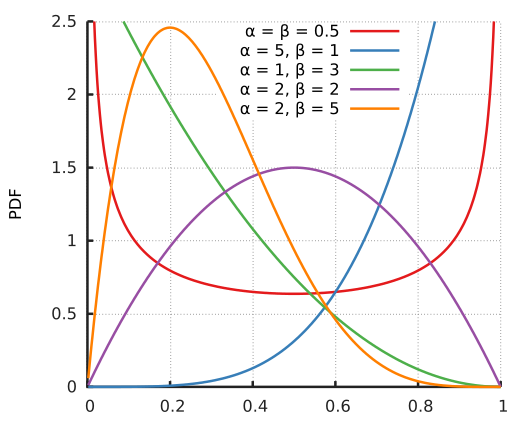
\includegraphics[width = .6\textwidth]{figures/beta}
\caption{Beta distribution probability density function. Lighter green indicates a more diffuse prior that can be interpreted as having fewer pseudocounts before seeing the data.}
\label{fig:beta}
\end{figure}

Because we often have some knowledge of $\pi$ before seeing the data, it is often helpful to assume a weakly informative prior, which will bias results toward the prior but improve efficiency. Researchers often mistakenly state that they have chosen a ``non-informative'' or ``flat'' prior. In our example, for instance, you might place a Beta(1,1) or uniform prior on $\pi$. This would be a reasonable choice, but it would not be flat if you reparameterized to focus on $\gamma = \pi^2$. Under this reparameterization, a uniform prior on $\pi$ would correspond to much greater prior probabilities on $\gamma$ near 0 than $\gamma$ near 1. Because priors can be sensitive to parameterization, one should be cautious in claiming that any prior is flat.

To avoid this problem, a common diffuse prior distribution is the \bgreen{Jeffreys prior}
$$f(\theta)\propto\sqrt{\underbrace{\left\lvert\mathcal{I}\left(\vec\theta\right)\right\rvert}_{\substack{\text{Determinant of}\\\text{Fisher information}}}}$$
The Jeffreys prior is invariant to reparameterizations of $\theta$ because the parameterization of $\theta$ is taken into account in the Fisher information. In the Bernoulli example, the Jeffreys prior is a $\text{Beta}\left(\frac{1}{2},\frac{1}{2}\right)$. The Jeffreys prior is still informative, however: the posterior mean in this case is biased toward $\frac{1}{2}$.

$$\hat\pi_\text{Posterior Mean} = 
	\E\left[\text{Beta}\left(\frac{1}{2}+ \sum_{i=1}^n y_i,\frac{1}{2} + n - \sum_{i=1}^n y_i\right)\right] = 
	\underbrace{\left(\frac{1}{2}\right)}_{\substack{\text{Prior}\\\text{mean}}}\left(\frac{1}{1+n}\right) + 
		\underbrace{\left(\frac{\sum_{i=1}^n y_i}{n}\right)}_{\hat\pi_\text{MLE}}\left(\frac{n}{1 + n}\right)$$
		
Rather than arguing about the choice of a flat prior, it may be wiser to choose a ``weakly informative'' prior which gains efficiency by placing lower probability on highly improbable regions of the parameter space \citep{gelman2008}. We chose a conjugate prior in this example so that the math would be nice, but one can use Markov Chain Monte Carlo (MCMC) methods to sample from the posterior distribution even when it does not have an analytical solution (see \citealt{brooks2011} and \citealt{robert2010} for introductions). MCMC represents one of the foremost computational breakthroughs in statistics in recent decades, and new methods for sampling from the posterior are continually being developed (i.e. \citealt{carpenter2017}). Bayesian methods are likely to become even more accessible to applied researchers in the future as computation improves. For those interested in Bayesian inference, we recommend \citet{hoff2009} and \citet{gelman2014}.

\newpage
\begin{small}
\bibliography{GLM_handout}
\end{small}

\end{document}
